% Created by tikzDevice version 0.12.6 on 2026-09-22 03:17:04
% !TEX encoding = UTF-8 Unicode
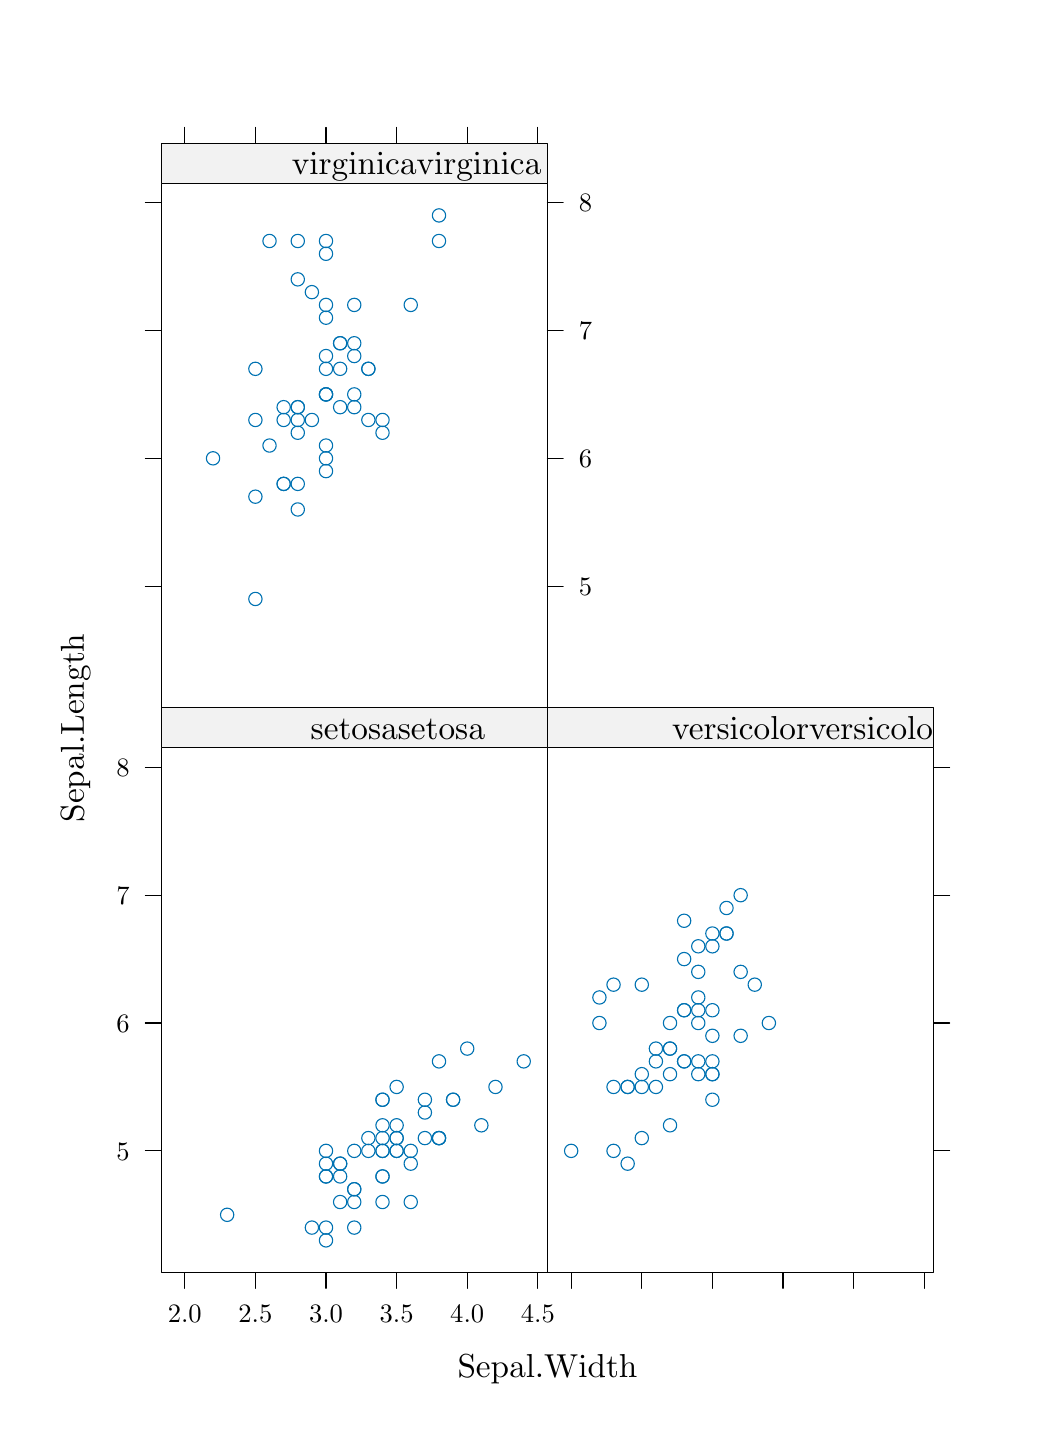
\begin{tikzpicture}[x=1pt,y=1pt]
\definecolor{fillColor}{RGB}{255,255,255}
\path[use as bounding box,fill=fillColor,fill opacity=0.00] (0,0) rectangle (361.35,505.89);
\begin{scope}
\path[clip] (  0.00,  0.00) rectangle (361.35,505.89);

\path[] (  0.00,  0.00) rectangle (361.35,505.89);
\definecolor{drawColor}{RGB}{0,0,0}

\node[text=drawColor,anchor=base,inner sep=0pt, outer sep=0pt, scale=  1.20] at (187.82, 18.07) {Sepal.Width};
\end{scope}
\begin{scope}
\path[clip] (  0.00,  0.00) rectangle (361.35,505.89);
\definecolor{drawColor}{RGB}{0,0,0}

\node[text=drawColor,rotate= 90.00,anchor=base,inner sep=0pt, outer sep=0pt, scale=  1.20] at ( 20.31,252.86) {Sepal.Length};
\end{scope}
\begin{scope}
\path[clip] (  0.00,  0.00) rectangle (361.35,505.89);
\definecolor{drawColor}{RGB}{0,0,0}

\path[draw=drawColor,line width= 0.4pt,line join=round,line cap=round] ( 48.20,100.02) -- ( 42.51,100.02);

\path[draw=drawColor,line width= 0.4pt,line join=round,line cap=round] ( 48.20,146.22) -- ( 42.51,146.22);

\path[draw=drawColor,line width= 0.4pt,line join=round,line cap=round] ( 48.20,192.41) -- ( 42.51,192.41);

\path[draw=drawColor,line width= 0.4pt,line join=round,line cap=round] ( 48.20,238.61) -- ( 42.51,238.61);

\node[text=drawColor,anchor=base east,inner sep=0pt, outer sep=0pt, scale=  0.96] at ( 36.82, 96.71) {5};

\node[text=drawColor,anchor=base east,inner sep=0pt, outer sep=0pt, scale=  0.96] at ( 36.82,142.91) {6};

\node[text=drawColor,anchor=base east,inner sep=0pt, outer sep=0pt, scale=  0.96] at ( 36.82,189.11) {7};

\node[text=drawColor,anchor=base east,inner sep=0pt, outer sep=0pt, scale=  0.96] at ( 36.82,235.31) {8};
\end{scope}
\begin{scope}
\path[clip] (  0.00,  0.00) rectangle (361.35,505.89);
\definecolor{drawColor}{RGB}{0,0,0}

\path[draw=drawColor,line width= 0.4pt,line join=round,line cap=round] ( 56.78, 56.04) -- ( 56.78, 50.35);

\path[draw=drawColor,line width= 0.4pt,line join=round,line cap=round] ( 82.29, 56.04) -- ( 82.29, 50.35);

\path[draw=drawColor,line width= 0.4pt,line join=round,line cap=round] (107.80, 56.04) -- (107.80, 50.35);

\path[draw=drawColor,line width= 0.4pt,line join=round,line cap=round] (133.32, 56.04) -- (133.32, 50.35);

\path[draw=drawColor,line width= 0.4pt,line join=round,line cap=round] (158.83, 56.04) -- (158.83, 50.35);

\path[draw=drawColor,line width= 0.4pt,line join=round,line cap=round] (184.35, 56.04) -- (184.35, 50.35);

\node[text=drawColor,anchor=base,inner sep=0pt, outer sep=0pt, scale=  0.96] at ( 56.78, 38.05) {2.0};

\node[text=drawColor,anchor=base,inner sep=0pt, outer sep=0pt, scale=  0.96] at ( 82.29, 38.05) {2.5};

\node[text=drawColor,anchor=base,inner sep=0pt, outer sep=0pt, scale=  0.96] at (107.80, 38.05) {3.0};

\node[text=drawColor,anchor=base,inner sep=0pt, outer sep=0pt, scale=  0.96] at (133.32, 38.05) {3.5};

\node[text=drawColor,anchor=base,inner sep=0pt, outer sep=0pt, scale=  0.96] at (158.83, 38.05) {4.0};

\node[text=drawColor,anchor=base,inner sep=0pt, outer sep=0pt, scale=  0.96] at (184.35, 38.05) {4.5};
\end{scope}
\begin{scope}
\path[clip] ( 48.20, 56.04) rectangle (187.82,245.63);
\definecolor{drawColor}{RGB}{0,114,178}

\path[draw=drawColor,line width= 0.4pt,line join=round,line cap=round] (133.32,104.64) circle (  2.41);

\path[draw=drawColor,line width= 0.4pt,line join=round,line cap=round] (107.80, 95.40) circle (  2.41);

\path[draw=drawColor,line width= 0.4pt,line join=round,line cap=round] (118.01, 86.16) circle (  2.41);

\path[draw=drawColor,line width= 0.4pt,line join=round,line cap=round] (112.91, 81.54) circle (  2.41);

\path[draw=drawColor,line width= 0.4pt,line join=round,line cap=round] (138.42,100.02) circle (  2.41);

\path[draw=drawColor,line width= 0.4pt,line join=round,line cap=round] (153.73,118.50) circle (  2.41);

\path[draw=drawColor,line width= 0.4pt,line join=round,line cap=round] (128.22, 81.54) circle (  2.41);

\path[draw=drawColor,line width= 0.4pt,line join=round,line cap=round] (128.22,100.02) circle (  2.41);

\path[draw=drawColor,line width= 0.4pt,line join=round,line cap=round] (102.70, 72.30) circle (  2.41);

\path[draw=drawColor,line width= 0.4pt,line join=round,line cap=round] (112.91, 95.40) circle (  2.41);

\path[draw=drawColor,line width= 0.4pt,line join=round,line cap=round] (143.53,118.50) circle (  2.41);

\path[draw=drawColor,line width= 0.4pt,line join=round,line cap=round] (128.22, 90.78) circle (  2.41);

\path[draw=drawColor,line width= 0.4pt,line join=round,line cap=round] (107.80, 90.78) circle (  2.41);

\path[draw=drawColor,line width= 0.4pt,line join=round,line cap=round] (107.80, 67.68) circle (  2.41);

\path[draw=drawColor,line width= 0.4pt,line join=round,line cap=round] (158.83,136.98) circle (  2.41);

\path[draw=drawColor,line width= 0.4pt,line join=round,line cap=round] (179.25,132.36) circle (  2.41);

\path[draw=drawColor,line width= 0.4pt,line join=round,line cap=round] (153.73,118.50) circle (  2.41);

\path[draw=drawColor,line width= 0.4pt,line join=round,line cap=round] (133.32,104.64) circle (  2.41);

\path[draw=drawColor,line width= 0.4pt,line join=round,line cap=round] (148.63,132.36) circle (  2.41);

\path[draw=drawColor,line width= 0.4pt,line join=round,line cap=round] (148.63,104.64) circle (  2.41);

\path[draw=drawColor,line width= 0.4pt,line join=round,line cap=round] (128.22,118.50) circle (  2.41);

\path[draw=drawColor,line width= 0.4pt,line join=round,line cap=round] (143.53,104.64) circle (  2.41);

\path[draw=drawColor,line width= 0.4pt,line join=round,line cap=round] (138.42, 81.54) circle (  2.41);

\path[draw=drawColor,line width= 0.4pt,line join=round,line cap=round] (123.11,104.64) circle (  2.41);

\path[draw=drawColor,line width= 0.4pt,line join=round,line cap=round] (128.22, 90.78) circle (  2.41);

\path[draw=drawColor,line width= 0.4pt,line join=round,line cap=round] (107.80,100.02) circle (  2.41);

\path[draw=drawColor,line width= 0.4pt,line join=round,line cap=round] (128.22,100.02) circle (  2.41);

\path[draw=drawColor,line width= 0.4pt,line join=round,line cap=round] (133.32,109.26) circle (  2.41);

\path[draw=drawColor,line width= 0.4pt,line join=round,line cap=round] (128.22,109.26) circle (  2.41);

\path[draw=drawColor,line width= 0.4pt,line join=round,line cap=round] (118.01, 86.16) circle (  2.41);

\path[draw=drawColor,line width= 0.4pt,line join=round,line cap=round] (112.91, 90.78) circle (  2.41);

\path[draw=drawColor,line width= 0.4pt,line join=round,line cap=round] (128.22,118.50) circle (  2.41);

\path[draw=drawColor,line width= 0.4pt,line join=round,line cap=round] (163.94,109.26) circle (  2.41);

\path[draw=drawColor,line width= 0.4pt,line join=round,line cap=round] (169.04,123.12) circle (  2.41);

\path[draw=drawColor,line width= 0.4pt,line join=round,line cap=round] (112.91, 95.40) circle (  2.41);

\path[draw=drawColor,line width= 0.4pt,line join=round,line cap=round] (118.01,100.02) circle (  2.41);

\path[draw=drawColor,line width= 0.4pt,line join=round,line cap=round] (133.32,123.12) circle (  2.41);

\path[draw=drawColor,line width= 0.4pt,line join=round,line cap=round] (138.42, 95.40) circle (  2.41);

\path[draw=drawColor,line width= 0.4pt,line join=round,line cap=round] (107.80, 72.30) circle (  2.41);

\path[draw=drawColor,line width= 0.4pt,line join=round,line cap=round] (128.22,104.64) circle (  2.41);

\path[draw=drawColor,line width= 0.4pt,line join=round,line cap=round] (133.32,100.02) circle (  2.41);

\path[draw=drawColor,line width= 0.4pt,line join=round,line cap=round] ( 72.08, 76.92) circle (  2.41);

\path[draw=drawColor,line width= 0.4pt,line join=round,line cap=round] (118.01, 72.30) circle (  2.41);

\path[draw=drawColor,line width= 0.4pt,line join=round,line cap=round] (133.32,100.02) circle (  2.41);

\path[draw=drawColor,line width= 0.4pt,line join=round,line cap=round] (148.63,104.64) circle (  2.41);

\path[draw=drawColor,line width= 0.4pt,line join=round,line cap=round] (107.80, 90.78) circle (  2.41);

\path[draw=drawColor,line width= 0.4pt,line join=round,line cap=round] (148.63,104.64) circle (  2.41);

\path[draw=drawColor,line width= 0.4pt,line join=round,line cap=round] (118.01, 81.54) circle (  2.41);

\path[draw=drawColor,line width= 0.4pt,line join=round,line cap=round] (143.53,113.88) circle (  2.41);

\path[draw=drawColor,line width= 0.4pt,line join=round,line cap=round] (123.11,100.02) circle (  2.41);
\end{scope}
\begin{scope}
\path[clip] (  0.00,  0.00) rectangle (361.35,505.89);
\definecolor{drawColor}{RGB}{0,0,0}

\path[draw=drawColor,line width= 0.4pt,line join=round,line cap=round] ( 48.20, 56.04) rectangle (187.82,245.63);
\end{scope}
\begin{scope}
\path[clip] ( 48.20,245.63) rectangle (187.82,260.09);
\definecolor{drawColor}{gray}{0.95}
\definecolor{fillColor}{gray}{0.95}

\path[draw=drawColor,line width= 0.4pt,line join=round,line cap=round,fill=fillColor] ( 48.20,245.63) rectangle (187.82,260.09);
\definecolor{drawColor}{RGB}{0,0,0}

\node[text=drawColor,anchor=base west,inner sep=0pt, outer sep=0pt, scale=  1.20] at (102.28,248.73) {\hyperlink{setosa}{setosa}};
\end{scope}
\begin{scope}
\path[clip] (  0.00,  0.00) rectangle (361.35,505.89);
\definecolor{drawColor}{RGB}{0,0,0}

\path[draw=drawColor,line width= 0.4pt,line join=round,line cap=round] ( 48.20,245.63) rectangle (187.82,260.09);
\end{scope}
\begin{scope}
\path[clip] (  0.00,  0.00) rectangle (361.35,505.89);
\definecolor{drawColor}{RGB}{0,0,0}

\path[draw=drawColor,line width= 0.4pt,line join=round,line cap=round] (196.39, 56.04) -- (196.39, 50.35);

\path[draw=drawColor,line width= 0.4pt,line join=round,line cap=round] (221.91, 56.04) -- (221.91, 50.35);

\path[draw=drawColor,line width= 0.4pt,line join=round,line cap=round] (247.42, 56.04) -- (247.42, 50.35);

\path[draw=drawColor,line width= 0.4pt,line join=round,line cap=round] (272.94, 56.04) -- (272.94, 50.35);

\path[draw=drawColor,line width= 0.4pt,line join=round,line cap=round] (298.45, 56.04) -- (298.45, 50.35);

\path[draw=drawColor,line width= 0.4pt,line join=round,line cap=round] (323.96, 56.04) -- (323.96, 50.35);

\path[draw=drawColor,line width= 0.4pt,line join=round,line cap=round] (327.43,100.02) -- (333.13,100.02);

\path[draw=drawColor,line width= 0.4pt,line join=round,line cap=round] (327.43,146.22) -- (333.13,146.22);

\path[draw=drawColor,line width= 0.4pt,line join=round,line cap=round] (327.43,192.41) -- (333.13,192.41);

\path[draw=drawColor,line width= 0.4pt,line join=round,line cap=round] (327.43,238.61) -- (333.13,238.61);
\end{scope}
\begin{scope}
\path[clip] (187.82, 56.04) rectangle (327.43,245.63);
\definecolor{drawColor}{RGB}{0,114,178}

\path[draw=drawColor,line width= 0.4pt,line join=round,line cap=round] (257.63,192.41) circle (  2.41);

\path[draw=drawColor,line width= 0.4pt,line join=round,line cap=round] (257.63,164.70) circle (  2.41);

\path[draw=drawColor,line width= 0.4pt,line join=round,line cap=round] (252.52,187.79) circle (  2.41);

\path[draw=drawColor,line width= 0.4pt,line join=round,line cap=round] (211.70,123.12) circle (  2.41);

\path[draw=drawColor,line width= 0.4pt,line join=round,line cap=round] (237.21,169.32) circle (  2.41);

\path[draw=drawColor,line width= 0.4pt,line join=round,line cap=round] (237.21,132.36) circle (  2.41);

\path[draw=drawColor,line width= 0.4pt,line join=round,line cap=round] (262.73,160.08) circle (  2.41);

\path[draw=drawColor,line width= 0.4pt,line join=round,line cap=round] (216.80, 95.40) circle (  2.41);

\path[draw=drawColor,line width= 0.4pt,line join=round,line cap=round] (242.32,173.94) circle (  2.41);

\path[draw=drawColor,line width= 0.4pt,line join=round,line cap=round] (232.11,109.26) circle (  2.41);

\path[draw=drawColor,line width= 0.4pt,line join=round,line cap=round] (196.39,100.02) circle (  2.41);

\path[draw=drawColor,line width= 0.4pt,line join=round,line cap=round] (247.42,141.60) circle (  2.41);

\path[draw=drawColor,line width= 0.4pt,line join=round,line cap=round] (206.60,146.22) circle (  2.41);

\path[draw=drawColor,line width= 0.4pt,line join=round,line cap=round] (242.32,150.84) circle (  2.41);

\path[draw=drawColor,line width= 0.4pt,line join=round,line cap=round] (242.32,127.74) circle (  2.41);

\path[draw=drawColor,line width= 0.4pt,line join=round,line cap=round] (252.52,178.56) circle (  2.41);

\path[draw=drawColor,line width= 0.4pt,line join=round,line cap=round] (247.42,127.74) circle (  2.41);

\path[draw=drawColor,line width= 0.4pt,line join=round,line cap=round] (232.11,136.98) circle (  2.41);

\path[draw=drawColor,line width= 0.4pt,line join=round,line cap=round] (206.60,155.46) circle (  2.41);

\path[draw=drawColor,line width= 0.4pt,line join=round,line cap=round] (221.91,127.74) circle (  2.41);

\path[draw=drawColor,line width= 0.4pt,line join=round,line cap=round] (257.63,141.60) circle (  2.41);

\path[draw=drawColor,line width= 0.4pt,line join=round,line cap=round] (237.21,150.84) circle (  2.41);

\path[draw=drawColor,line width= 0.4pt,line join=round,line cap=round] (221.91,160.08) circle (  2.41);

\path[draw=drawColor,line width= 0.4pt,line join=round,line cap=round] (237.21,150.84) circle (  2.41);

\path[draw=drawColor,line width= 0.4pt,line join=round,line cap=round] (242.32,164.70) circle (  2.41);

\path[draw=drawColor,line width= 0.4pt,line join=round,line cap=round] (247.42,173.94) circle (  2.41);

\path[draw=drawColor,line width= 0.4pt,line join=round,line cap=round] (237.21,183.17) circle (  2.41);

\path[draw=drawColor,line width= 0.4pt,line join=round,line cap=round] (247.42,178.56) circle (  2.41);

\path[draw=drawColor,line width= 0.4pt,line join=round,line cap=round] (242.32,146.22) circle (  2.41);

\path[draw=drawColor,line width= 0.4pt,line join=round,line cap=round] (227.01,132.36) circle (  2.41);

\path[draw=drawColor,line width= 0.4pt,line join=round,line cap=round] (216.80,123.12) circle (  2.41);

\path[draw=drawColor,line width= 0.4pt,line join=round,line cap=round] (216.80,123.12) circle (  2.41);

\path[draw=drawColor,line width= 0.4pt,line join=round,line cap=round] (232.11,136.98) circle (  2.41);

\path[draw=drawColor,line width= 0.4pt,line join=round,line cap=round] (232.11,146.22) circle (  2.41);

\path[draw=drawColor,line width= 0.4pt,line join=round,line cap=round] (247.42,118.50) circle (  2.41);

\path[draw=drawColor,line width= 0.4pt,line join=round,line cap=round] (267.83,146.22) circle (  2.41);

\path[draw=drawColor,line width= 0.4pt,line join=round,line cap=round] (252.52,178.56) circle (  2.41);

\path[draw=drawColor,line width= 0.4pt,line join=round,line cap=round] (211.70,160.08) circle (  2.41);

\path[draw=drawColor,line width= 0.4pt,line join=round,line cap=round] (247.42,127.74) circle (  2.41);

\path[draw=drawColor,line width= 0.4pt,line join=round,line cap=round] (221.91,123.12) circle (  2.41);

\path[draw=drawColor,line width= 0.4pt,line join=round,line cap=round] (227.01,123.12) circle (  2.41);

\path[draw=drawColor,line width= 0.4pt,line join=round,line cap=round] (247.42,150.84) circle (  2.41);

\path[draw=drawColor,line width= 0.4pt,line join=round,line cap=round] (227.01,136.98) circle (  2.41);

\path[draw=drawColor,line width= 0.4pt,line join=round,line cap=round] (211.70,100.02) circle (  2.41);

\path[draw=drawColor,line width= 0.4pt,line join=round,line cap=round] (232.11,127.74) circle (  2.41);

\path[draw=drawColor,line width= 0.4pt,line join=round,line cap=round] (247.42,132.36) circle (  2.41);

\path[draw=drawColor,line width= 0.4pt,line join=round,line cap=round] (242.32,132.36) circle (  2.41);

\path[draw=drawColor,line width= 0.4pt,line join=round,line cap=round] (242.32,155.46) circle (  2.41);

\path[draw=drawColor,line width= 0.4pt,line join=round,line cap=round] (221.91,104.64) circle (  2.41);

\path[draw=drawColor,line width= 0.4pt,line join=round,line cap=round] (237.21,132.36) circle (  2.41);
\end{scope}
\begin{scope}
\path[clip] (  0.00,  0.00) rectangle (361.35,505.89);
\definecolor{drawColor}{RGB}{0,0,0}

\path[draw=drawColor,line width= 0.4pt,line join=round,line cap=round] (187.82, 56.04) rectangle (327.43,245.63);
\end{scope}
\begin{scope}
\path[clip] (187.82,245.63) rectangle (327.43,260.09);
\definecolor{drawColor}{gray}{0.95}
\definecolor{fillColor}{gray}{0.95}

\path[draw=drawColor,line width= 0.4pt,line join=round,line cap=round,fill=fillColor] (187.82,245.63) rectangle (327.43,260.09);
\definecolor{drawColor}{RGB}{0,0,0}

\node[text=drawColor,anchor=base west,inner sep=0pt, outer sep=0pt, scale=  1.20] at (232.90,248.73) {\hyperlink{versicolor}{versicolor}};
\end{scope}
\begin{scope}
\path[clip] (  0.00,  0.00) rectangle (361.35,505.89);
\definecolor{drawColor}{RGB}{0,0,0}

\path[draw=drawColor,line width= 0.4pt,line join=round,line cap=round] (187.82,245.63) rectangle (327.43,260.09);
\end{scope}
\begin{scope}
\path[clip] (  0.00,  0.00) rectangle (361.35,505.89);
\definecolor{drawColor}{RGB}{0,0,0}

\path[draw=drawColor,line width= 0.4pt,line join=round,line cap=round] ( 56.78,464.14) -- ( 56.78,469.83);

\path[draw=drawColor,line width= 0.4pt,line join=round,line cap=round] ( 82.29,464.14) -- ( 82.29,469.83);

\path[draw=drawColor,line width= 0.4pt,line join=round,line cap=round] (107.80,464.14) -- (107.80,469.83);

\path[draw=drawColor,line width= 0.4pt,line join=round,line cap=round] (133.32,464.14) -- (133.32,469.83);

\path[draw=drawColor,line width= 0.4pt,line join=round,line cap=round] (158.83,464.14) -- (158.83,469.83);

\path[draw=drawColor,line width= 0.4pt,line join=round,line cap=round] (184.35,464.14) -- (184.35,469.83);
\end{scope}
\begin{scope}
\path[clip] (  0.00,  0.00) rectangle (361.35,505.89);
\definecolor{drawColor}{RGB}{0,0,0}

\path[draw=drawColor,line width= 0.4pt,line join=round,line cap=round] ( 48.20,304.07) -- ( 42.51,304.07);

\path[draw=drawColor,line width= 0.4pt,line join=round,line cap=round] ( 48.20,350.27) -- ( 42.51,350.27);

\path[draw=drawColor,line width= 0.4pt,line join=round,line cap=round] ( 48.20,396.47) -- ( 42.51,396.47);

\path[draw=drawColor,line width= 0.4pt,line join=round,line cap=round] ( 48.20,442.66) -- ( 42.51,442.66);
\end{scope}
\begin{scope}
\path[clip] (  0.00,  0.00) rectangle (361.35,505.89);
\definecolor{drawColor}{RGB}{0,0,0}

\path[draw=drawColor,line width= 0.4pt,line join=round,line cap=round] (187.82,304.07) -- (193.51,304.07);

\path[draw=drawColor,line width= 0.4pt,line join=round,line cap=round] (187.82,350.27) -- (193.51,350.27);

\path[draw=drawColor,line width= 0.4pt,line join=round,line cap=round] (187.82,396.47) -- (193.51,396.47);

\path[draw=drawColor,line width= 0.4pt,line join=round,line cap=round] (187.82,442.66) -- (193.51,442.66);

\node[text=drawColor,anchor=base west,inner sep=0pt, outer sep=0pt, scale=  0.96] at (199.20,300.76) {5};

\node[text=drawColor,anchor=base west,inner sep=0pt, outer sep=0pt, scale=  0.96] at (199.20,346.96) {6};

\node[text=drawColor,anchor=base west,inner sep=0pt, outer sep=0pt, scale=  0.96] at (199.20,393.16) {7};

\node[text=drawColor,anchor=base west,inner sep=0pt, outer sep=0pt, scale=  0.96] at (199.20,439.36) {8};
\end{scope}
\begin{scope}
\path[clip] ( 48.20,260.09) rectangle (187.82,449.69);
\definecolor{drawColor}{RGB}{0,114,178}

\path[draw=drawColor,line width= 0.4pt,line join=round,line cap=round] (123.11,364.13) circle (  2.41);

\path[draw=drawColor,line width= 0.4pt,line join=round,line cap=round] ( 92.50,341.03) circle (  2.41);

\path[draw=drawColor,line width= 0.4pt,line join=round,line cap=round] (107.80,401.08) circle (  2.41);

\path[draw=drawColor,line width= 0.4pt,line join=round,line cap=round] (102.70,364.13) circle (  2.41);

\path[draw=drawColor,line width= 0.4pt,line join=round,line cap=round] (107.80,373.37) circle (  2.41);

\path[draw=drawColor,line width= 0.4pt,line join=round,line cap=round] (107.80,424.18) circle (  2.41);

\path[draw=drawColor,line width= 0.4pt,line join=round,line cap=round] ( 82.29,299.45) circle (  2.41);

\path[draw=drawColor,line width= 0.4pt,line join=round,line cap=round] (102.70,410.32) circle (  2.41);

\path[draw=drawColor,line width= 0.4pt,line join=round,line cap=round] ( 82.29,382.61) circle (  2.41);

\path[draw=drawColor,line width= 0.4pt,line join=round,line cap=round] (138.42,405.70) circle (  2.41);

\path[draw=drawColor,line width= 0.4pt,line join=round,line cap=round] (118.01,373.37) circle (  2.41);

\path[draw=drawColor,line width= 0.4pt,line join=round,line cap=round] ( 92.50,368.75) circle (  2.41);

\path[draw=drawColor,line width= 0.4pt,line join=round,line cap=round] (107.80,387.23) circle (  2.41);

\path[draw=drawColor,line width= 0.4pt,line join=round,line cap=round] ( 82.29,336.41) circle (  2.41);

\path[draw=drawColor,line width= 0.4pt,line join=round,line cap=round] ( 97.60,341.03) circle (  2.41);

\path[draw=drawColor,line width= 0.4pt,line join=round,line cap=round] (118.01,368.75) circle (  2.41);

\path[draw=drawColor,line width= 0.4pt,line join=round,line cap=round] (107.80,373.37) circle (  2.41);

\path[draw=drawColor,line width= 0.4pt,line join=round,line cap=round] (148.63,428.80) circle (  2.41);

\path[draw=drawColor,line width= 0.4pt,line join=round,line cap=round] ( 87.39,428.80) circle (  2.41);

\path[draw=drawColor,line width= 0.4pt,line join=round,line cap=round] ( 66.98,350.27) circle (  2.41);

\path[draw=drawColor,line width= 0.4pt,line join=round,line cap=round] (118.01,391.85) circle (  2.41);

\path[draw=drawColor,line width= 0.4pt,line join=round,line cap=round] ( 97.60,331.79) circle (  2.41);

\path[draw=drawColor,line width= 0.4pt,line join=round,line cap=round] ( 97.60,428.80) circle (  2.41);

\path[draw=drawColor,line width= 0.4pt,line join=round,line cap=round] ( 92.50,364.13) circle (  2.41);

\path[draw=drawColor,line width= 0.4pt,line join=round,line cap=round] (123.11,382.61) circle (  2.41);

\path[draw=drawColor,line width= 0.4pt,line join=round,line cap=round] (118.01,405.70) circle (  2.41);

\path[draw=drawColor,line width= 0.4pt,line join=round,line cap=round] ( 97.60,359.51) circle (  2.41);

\path[draw=drawColor,line width= 0.4pt,line join=round,line cap=round] (107.80,354.89) circle (  2.41);

\path[draw=drawColor,line width= 0.4pt,line join=round,line cap=round] ( 97.60,368.75) circle (  2.41);

\path[draw=drawColor,line width= 0.4pt,line join=round,line cap=round] (107.80,405.70) circle (  2.41);

\path[draw=drawColor,line width= 0.4pt,line join=round,line cap=round] ( 97.60,414.94) circle (  2.41);

\path[draw=drawColor,line width= 0.4pt,line join=round,line cap=round] (148.63,438.04) circle (  2.41);

\path[draw=drawColor,line width= 0.4pt,line join=round,line cap=round] ( 97.60,368.75) circle (  2.41);

\path[draw=drawColor,line width= 0.4pt,line join=round,line cap=round] ( 97.60,364.13) circle (  2.41);

\path[draw=drawColor,line width= 0.4pt,line join=round,line cap=round] ( 87.39,354.89) circle (  2.41);

\path[draw=drawColor,line width= 0.4pt,line join=round,line cap=round] (107.80,428.80) circle (  2.41);

\path[draw=drawColor,line width= 0.4pt,line join=round,line cap=round] (128.22,364.13) circle (  2.41);

\path[draw=drawColor,line width= 0.4pt,line join=round,line cap=round] (112.91,368.75) circle (  2.41);

\path[draw=drawColor,line width= 0.4pt,line join=round,line cap=round] (107.80,350.27) circle (  2.41);

\path[draw=drawColor,line width= 0.4pt,line join=round,line cap=round] (112.91,391.85) circle (  2.41);

\path[draw=drawColor,line width= 0.4pt,line join=round,line cap=round] (112.91,382.61) circle (  2.41);

\path[draw=drawColor,line width= 0.4pt,line join=round,line cap=round] (112.91,391.85) circle (  2.41);

\path[draw=drawColor,line width= 0.4pt,line join=round,line cap=round] ( 92.50,341.03) circle (  2.41);

\path[draw=drawColor,line width= 0.4pt,line join=round,line cap=round] (118.01,387.23) circle (  2.41);

\path[draw=drawColor,line width= 0.4pt,line join=round,line cap=round] (123.11,382.61) circle (  2.41);

\path[draw=drawColor,line width= 0.4pt,line join=round,line cap=round] (107.80,382.61) circle (  2.41);

\path[draw=drawColor,line width= 0.4pt,line join=round,line cap=round] ( 82.29,364.13) circle (  2.41);

\path[draw=drawColor,line width= 0.4pt,line join=round,line cap=round] (107.80,373.37) circle (  2.41);

\path[draw=drawColor,line width= 0.4pt,line join=round,line cap=round] (128.22,359.51) circle (  2.41);

\path[draw=drawColor,line width= 0.4pt,line join=round,line cap=round] (107.80,345.65) circle (  2.41);
\end{scope}
\begin{scope}
\path[clip] (  0.00,  0.00) rectangle (361.35,505.89);
\definecolor{drawColor}{RGB}{0,0,0}

\path[draw=drawColor,line width= 0.4pt,line join=round,line cap=round] ( 48.20,260.09) rectangle (187.82,449.69);
\end{scope}
\begin{scope}
\path[clip] ( 48.20,449.69) rectangle (187.82,464.14);
\definecolor{drawColor}{gray}{0.95}
\definecolor{fillColor}{gray}{0.95}

\path[draw=drawColor,line width= 0.4pt,line join=round,line cap=round,fill=fillColor] ( 48.20,449.69) rectangle (187.82,464.14);
\definecolor{drawColor}{RGB}{0,0,0}

\node[text=drawColor,anchor=base west,inner sep=0pt, outer sep=0pt, scale=  1.20] at ( 95.50,452.78) {\hyperlink{virginica}{virginica}};
\end{scope}
\begin{scope}
\path[clip] (  0.00,  0.00) rectangle (361.35,505.89);
\definecolor{drawColor}{RGB}{0,0,0}

\path[draw=drawColor,line width= 0.4pt,line join=round,line cap=round] ( 48.20,449.69) rectangle (187.82,464.14);
\end{scope}
\end{tikzpicture}
